% !TEX root = ../main.tex

\section{Design and implementation}

\subsection{Pre-process data}
\begin{frame}{\insertsubsec}
  \begin{itemize}
    \item Pre-process image data
    \item Pre-process scalar data
    \item Generate pairs for training
  \end{itemize}

  \vspace{.5cm}
  Only 490 of the initial 671 could be used to fit a model because we needed the following 
  requirements:
  \begin{itemize}
    \item CT scan
    \item Tumour annotations
    \item Radiomic features
    \item Clinical information
  \end{itemize}
\end{frame}

\begin{frame}{Image data pre-processing}
  \begin{figure}
    \centering
    \scalebox{.6}{\def\customimage{10em}
\begin{tikzpicture}[node distance = 2]
    \node (P-0) at (0, 0) {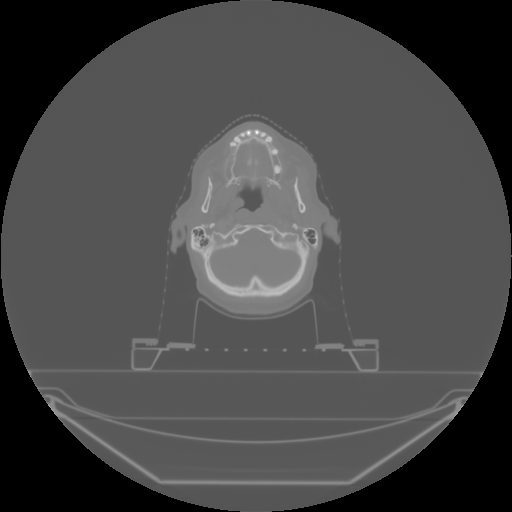
\includegraphics[width=\customimage]{images/preprocess/process_0}};
    \node [below = of P-0] (P-1) {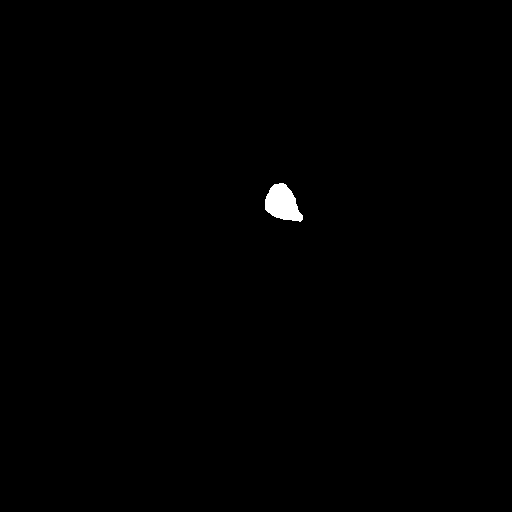
\includegraphics[width=\customimage]{images/preprocess/process_1}};

    \node [below = .2 of P-0] (text-0) {Scan};
    \node [below = .2 of P-1] (text-1) {Mask};
    
    \node [right = of P-1] (P-2-0) {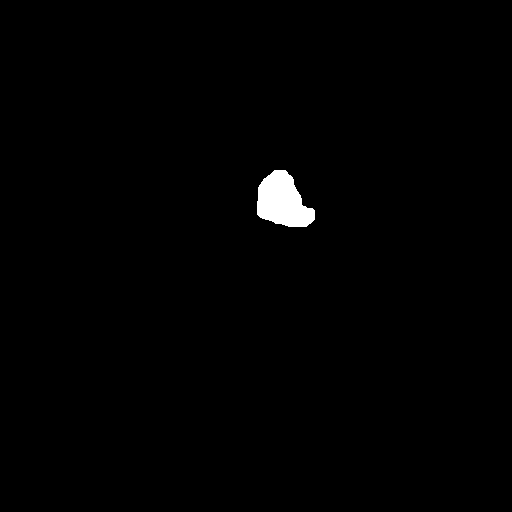
\includegraphics[width=\customimage]{images/preprocess/process_2_0}};
    \node [right = of P-2-0] (P-2-1) {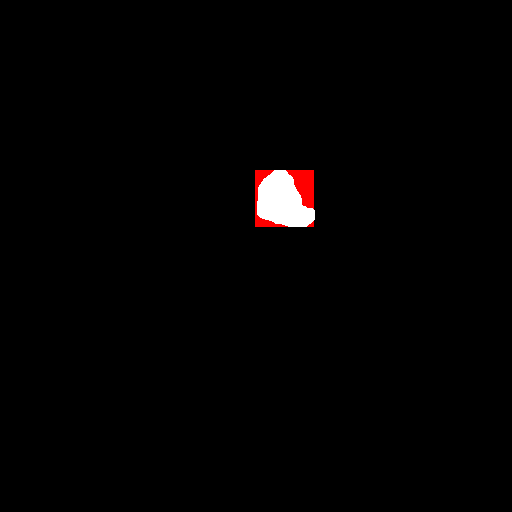
\includegraphics[width=\customimage]{images/preprocess/process_2_1}};
    \node [right = of P-2-1] (P-5) {
\includegraphics[width=\customimage]{images/preprocess/process_5}};
    
    \node [above = of P-2-1] (P-3) {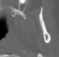
\includegraphics[width=\customimage]{images/preprocess/process_3}};
    \node [right = of P-3] (P-4) {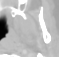
\includegraphics[width=\customimage]{images/preprocess/process_4}};

    \node [right = .5 of P-5, circle, draw] (prod) { \Large \( \times \) };
    
    \node [below = of P-5] (P-6) {
\includegraphics[width=\customimage]{images/preprocess/process_6}};
    \node [left = of P-6] (P-7) {
\includegraphics[width=\customimage]{images/preprocess/process_7}};
    \node [left = of P-7] (P-8) {
\includegraphics[width=\customimage]{images/preprocess/process_8}};

    \node [below = .2 of P-6] { \( 59 \times 57 \) px};
    \node [below = .2 of P-7] { \( 64 \times 64 \) px};
    \node [below = .2 of P-8] { \( 64 \times 64 \) px};

    \draw [-latex] (P-0) -- (P-3);
    \draw [-latex] (P-3) -- (P-4) node[midway, below, align=center] {Remove \\ extreme \\ values};
    \draw [-latex] (P-4) -| (prod);

    \draw [-latex] (P-1) -- (P-2-0) node[midway, below, align=center] {Gaussian \\ filter};
    \draw [-latex] (P-2-0) -- (P-2-1) node[midway, below, align=center] {Bounding \\ box};
    \draw [-latex] (P-2-1) -- (P-3) node[midway, right, align=center] {Slice};
    \draw [-latex] (P-2-1) -- (P-5) node[midway, below, align=center] {Slice};
    \draw [-latex] (P-5) -- (prod);

    \draw [-latex] (prod) |- (P-6) node[near end, below, align=center] {Apply \\ mask};
    \draw [-latex] (P-6) -- (P-7) node[midway, below, align=center] {
        Resize \\ \( 64 \times 64 \times 64 \)
    };

    \draw [-latex] (P-7) -- (P-8) node[midway, below, align=center] {Normalize};

\end{tikzpicture}}
    \caption{Image data pre-processing}
  \end{figure}
\end{frame}

\begin{frame}{Scalar data pre-processing}
  \begin{itemize}
    \item Clinical information
    \begin{itemize}
      \item Patient's ID
      \item Age
      \item Sex
      \item Survival event
      \item Survival time
    \end{itemize}
    \item Radiomic features, up to 725
    \begin{itemize}
      \item Tumour shape
      \item Intensity
      \item Volume
      \item ...
    \end{itemize}
  \end{itemize}
\end{frame}
\begin{frame}
  \begin{figure}
    \centering
    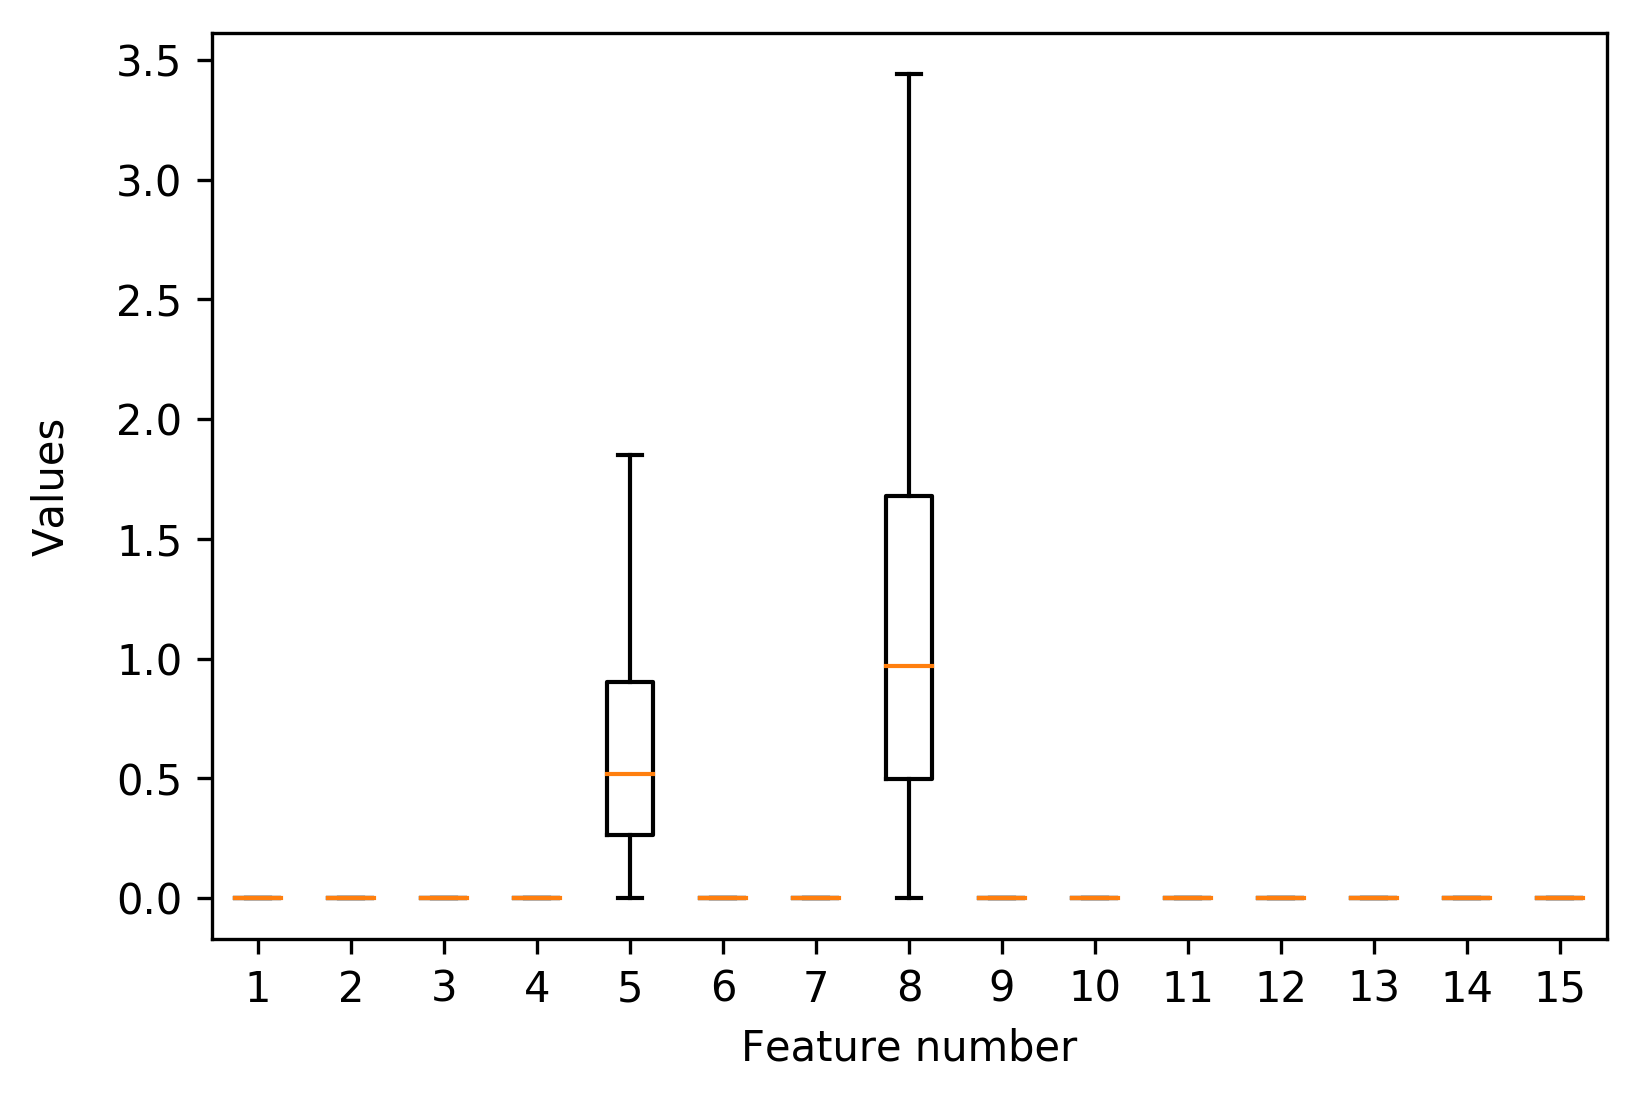
\includegraphics[width=\textwidth]{images/features_original}
    \caption{Features before normalization}
  \end{figure}
\end{frame}
\begin{frame}
  \begin{figure}
    \centering
    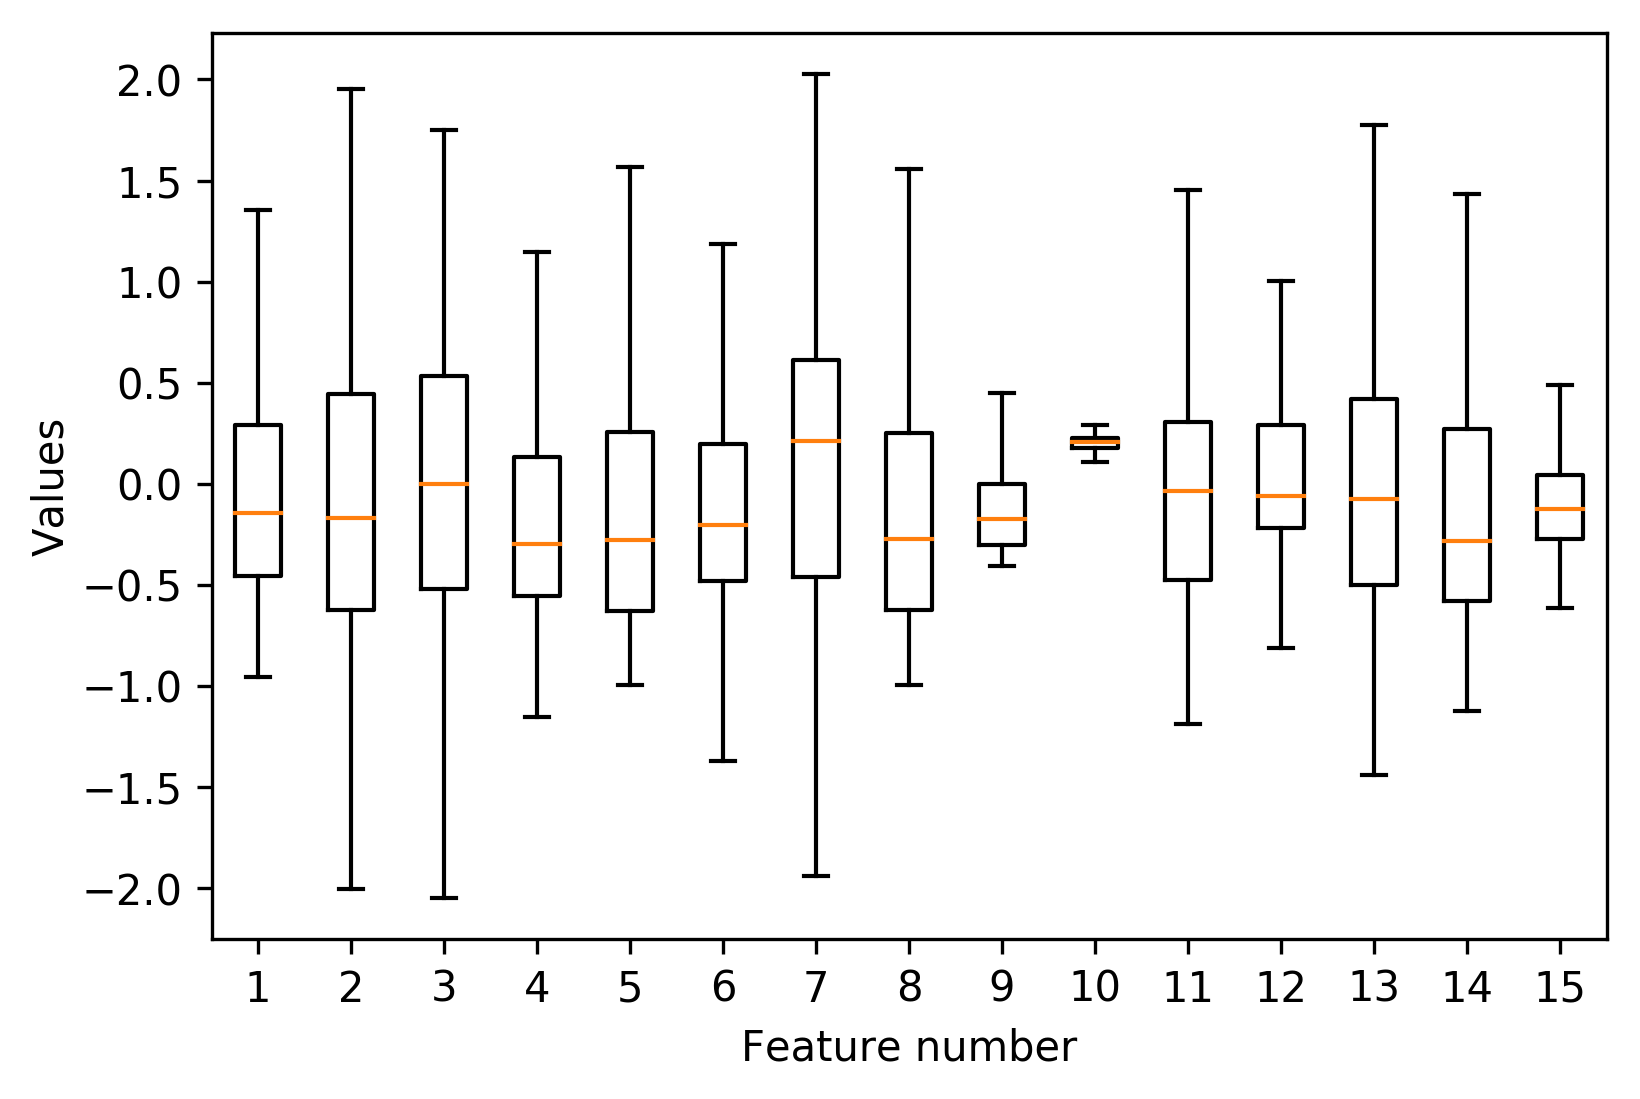
\includegraphics[width=\textwidth]{images/features_normalized}
    \caption{Features after normalization}
  \end{figure}
\end{frame}

\begin{frame}{Pair generation}
  
  \begin{figure}
    \centering
    \scalebox{.7}{\def\customimage{5em}
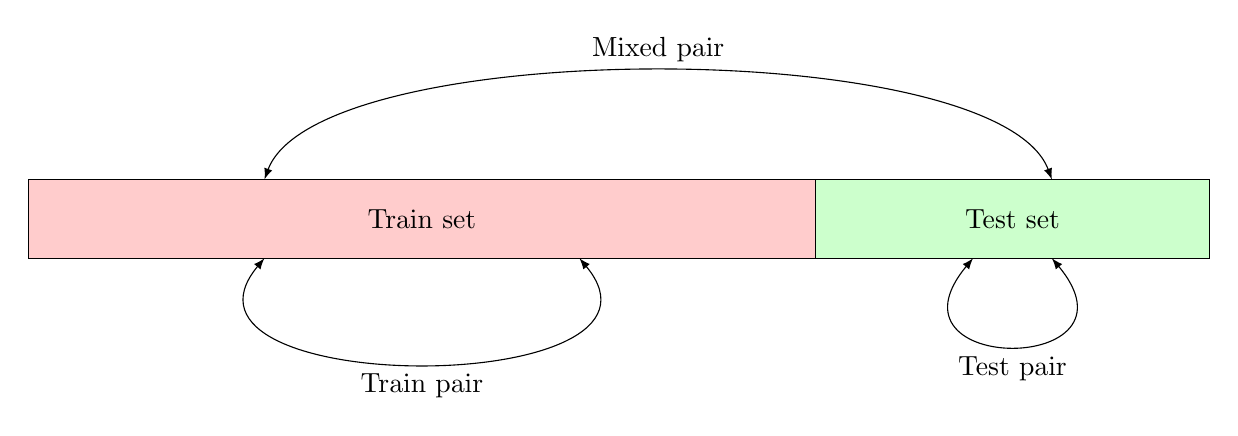
\begin{tikzpicture}
    
    \draw [fill = red!20] (0, 0) rectangle (10, 1);
    \draw [fill = green!20] (10, 0) rectangle (15, 1);

    \node at (5, .5) {Train set};
    \node at (12.5, .5) {Test set};

    \draw [bend right=130, latex-latex, looseness=1.5] (3, 0) to node [midway, below] {Train pair} (7, 0);
    \draw [bend right=130, latex-latex, looseness=5] (12, 0) to node [midway, below] {Test pair} (13, 0);
    \draw [bend left=70, latex-latex, looseness=.5] (3, 1) to node [midway, above] {Mixed pair} (13, 1);
\end{tikzpicture}}
    \caption{Types of pairs generated from train and test sets}
  \end{figure}

  \begin{block}{Conditions}
    \begin{itemize}
      \item Both of them are uncensored \( E_A = E_B = 1 \)
      \item The uncensored time of one is smaller than the censored time of the other
            \( T_A < T_B | E_A = 1; E_B = 0 \)
    \end{itemize}
  \end{block}
\end{frame}

